%% This is an example first chapter.  You should put chapter/appendix that you
%% write into a separate file, and add a line \include{yourfilename} to
%% main.tex, where `yourfilename.tex' is the name of the chapter/appendix file.
%% You can process specific files by typing their names in at the 
%% \files=
%% prompt when you run the file main.tex through LaTeX.
\chapter{Metode Prediksi} \label{chap:prediksi}

% Bab ini akan membahas deretan menu yang ada di bagian atas halaman Ijah Webserver.

% \begin{figure}[H]
% 	\centering
% 	
\includegraphics[scale=0.3]{ijah_menu_top.png}
% 	\caption{Deretan Menu pada Ijah Webserver}
% 	\label{fig:ijah_menu_top}
% \end{figure}

% \section{Manual}

% Menu \emph{Manual} berisi \emph{link} untuk mendownload file Manual penggunaan Ijah Webserver. Kedepannya, isi file Manual juga akan ditampilkan di halaman ini.

% \begin{figure}[H]
% 	\centering
% 	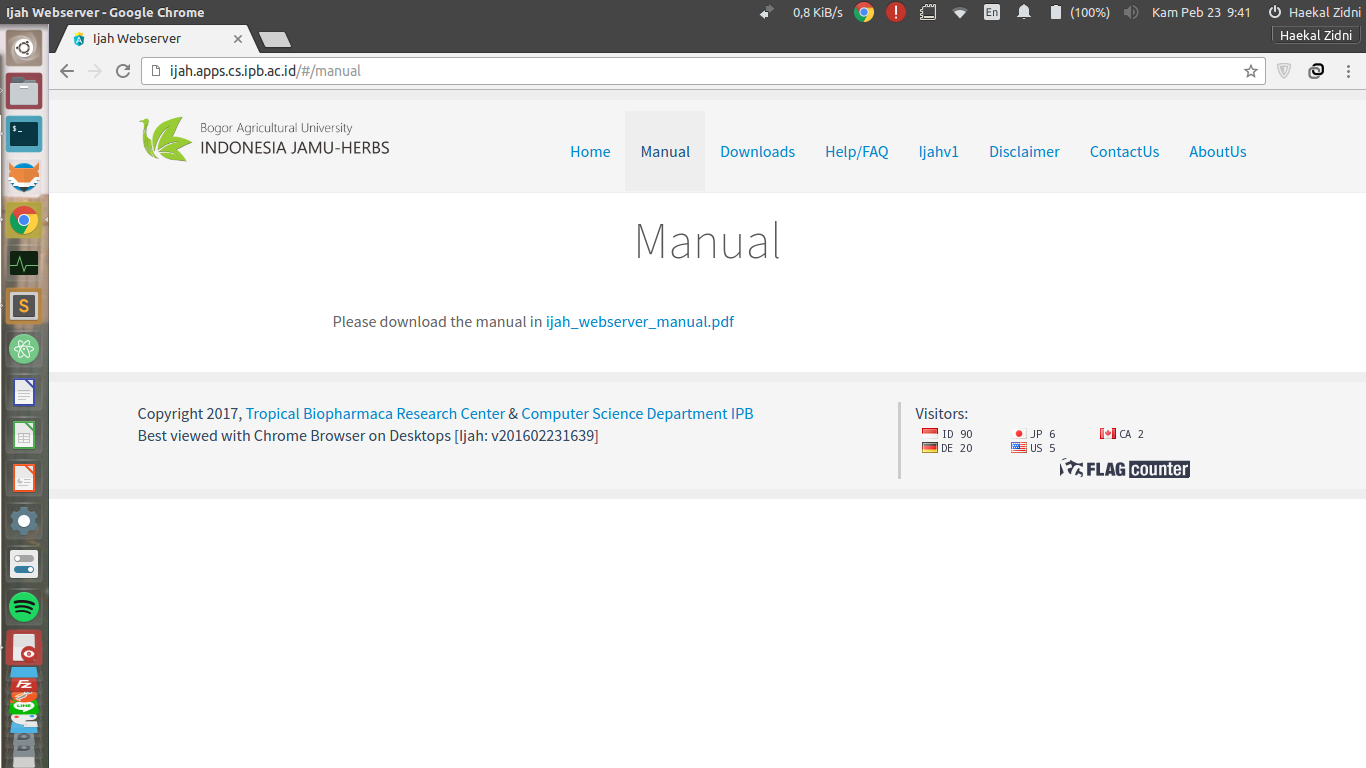
\includegraphics[scale=0.3]{ijah_manual_page.png}
% 	\caption{Halaman Manual}
% 	\label{fig:ijah_manual_page}
% \end{figure}

% \section{Downloads} \label{Downloads}

% Menu \emph{Downloads} menyediakan link untuk mengunduh Metadata seluruh item (tanaman, senyawa, protein, dan penyakit) yang ada dalam database Ijah Webserver. Juga disediakan data seluruh konektivitas (keterhubungan) antar item dan data lainnya seperti similarity data, data sekuens protein, dan lain lain.

% Untuk mengunduh file pada halaman ini cukup klik nama file yang ingin diunduh

% \begin{figure}[H]
% 	\centering
% 	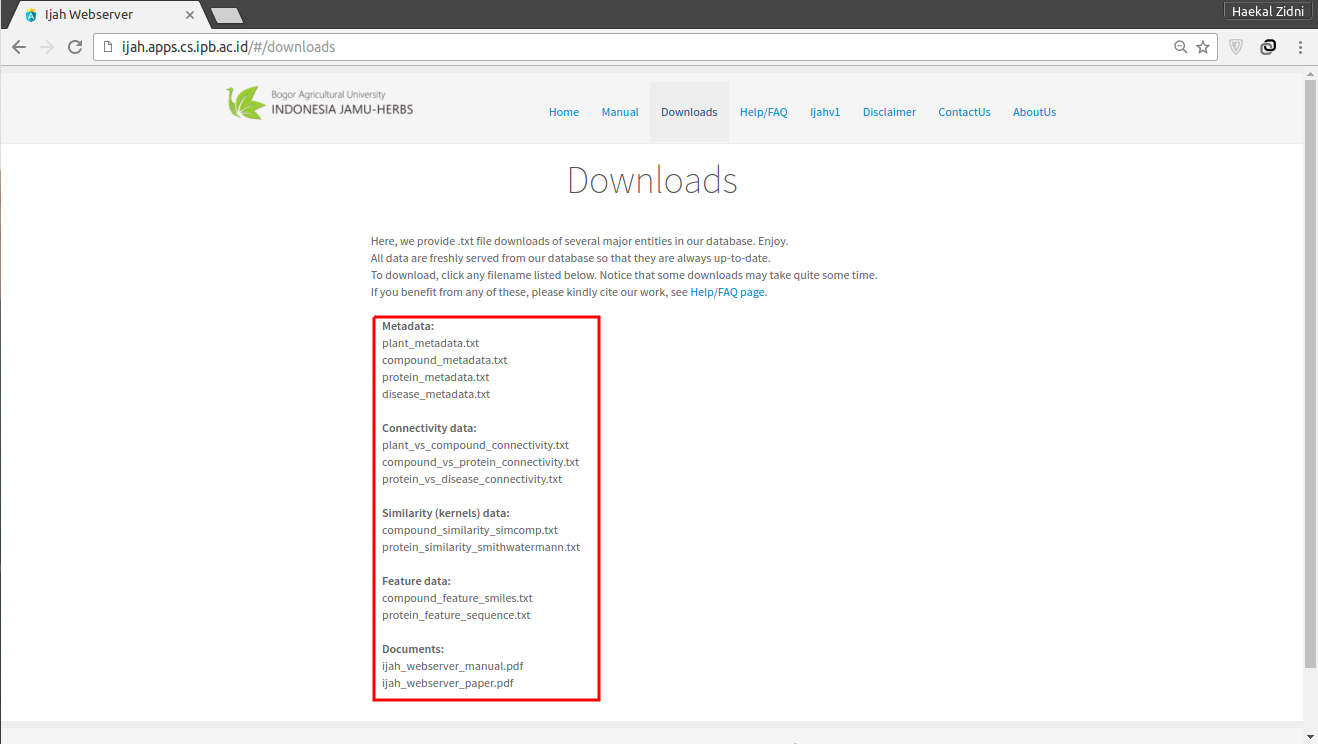
\includegraphics[scale=0.3]{ijah_downloadpage.png}
% 	\caption{Daftar file yang dapat di\-download}
% 	\label{fig:ijah_downloadpage}
% \end{figure}

% \subsection{Metadata}
% File yang dapat didownload pada kategori Metadata yaitu:

% \begin{itemize}
% \item \textbf{plant\_metadata.txt} -- Berisi metadata seluruh tanaman pada \emph{database} Ijah Webserver. 
% \item \textbf{compound\_metadata.txt} -- Berisi metadata seluruh senyawa (\emph{compound}) pada \emph{database} Ijah Webserver.
% \item \textbf{protein\_metadata.txt} -- Berisi metadata seluruh bioprotein pada \emph{database} Ijah Webserver.
% \item \textbf{disease\_metadata.txt} -- Berisi metadata seluruh penyakit pada \emph{database} Ijah Webserver.
% \end{itemize}

% \subsection{Connectivity Data}
% File yang dapat didownload pada kategori Connectivity Data yaitu:

% \begin{itemize}
% \item \textbf{plant\_vs\_compound\_connectivity.txt} -- Berisi data konektivitas tanaman dengan senyawa beserta skor konektivitasnya pada \emph{database} Ijah Webserver.
% \item \textbf{compound\_vs\_protein\_connectivity.txt} -- Berisi data konektivitas senyawa dengan protein beserta skor konektivitasnya pada \emph{database} Ijah Webserver.
% \item \textbf{protein\_vs\_disease\_connectivity.txt} -- Berisi data konektivitas protein dengan penyakit beserta skor konektivitasnya pada \emph{database} Ijah Webserver.
% \end{itemize}

% \subsection{Similarity (kernels) data}
% \begin{itemize}
% \item compound\_similarity\_simcomp.txt  
% \item protein\_similarity\_smithwatermann.txt  
% \end{itemize}

% \subsection{Feature data}
% \begin{itemize}
% \item compound\_feature\_smiles.txt  
% \item protein\_feature\_sequence.txt  
% \end{itemize}

% \subsection{Documents}
% Dokumentasi Ijah Webserver
% \begin{itemize}
% \item \textbf{ijah\_webserver\_manual.pdf} -- Manual penggunaan Ijah Webserver
% \item \textbf{ijah\_webserver\_paper.pdf} -- Paper penelitian Ijah Webserver
% \end{itemize}

% \section{Help/FAQ}
% Menu \emph{Help/FAQ} berisikan beberapa pertanyaan umum \emph{(Frequently Asked Questions)} beserta jawabannya. 

% \begin{figure}[H]
% 	\centering
% 	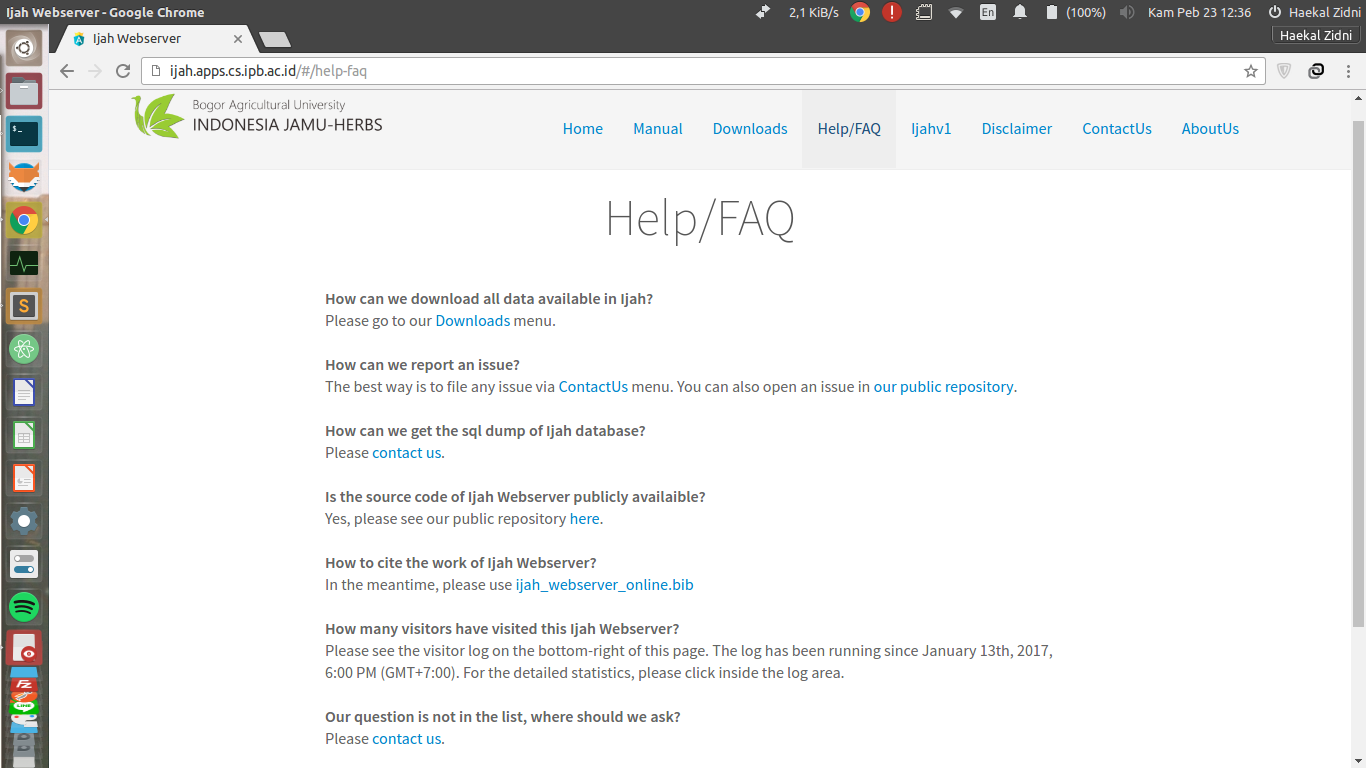
\includegraphics[scale=0.3]{ijah_faq.png}
% 	\caption{Halaman Help/FAQ}
% 	\label{fig:ijah_faq}
% \end{figure}

% Pertanyaan pertanyaan tersebut yaitu:

% \textbf{Q:} Bagaimana cara mengunduh semua data yang tersedia pada Ijah?

% A: Silakan lihat pada menu \nameref{Downloads}.

% \textbf{Q:} Bagaimana cara melaporkan isu atau galat?

% A: Silakan laporkan pada menu \nameref{Contact Us} atau pada \href{https://github.com/tttor/csipb-jamu-prj}{\emph{repository} publik kami}.

% \textbf{Q:} Bagaimana cara mendapatkan SQL dump dari database Ijah?

% A: Silakan kontak kami melalui menu \nameref{Contact Us}.

% \textbf{Q:} Apakah \emph{source code} Ijah tersedia secara publik?

% A: Ya, ada pada \href{https://github.com/tttor/csipb-jamu-prj}{\emph{repository} publik kami}.

% \textbf{Q:} Bagaimana cara mengutip dari paper Ijah Webserver?

% A: Silakan merujuk ke \href{http://ijah.apps.cs.ipb.ac.id/api/ijah_webserver_online.bib}{ijah\_webserver\_online.bib}.

% \textbf{Q:} Berapa banyak kunjungan ke Ijah Webserver?

% A: Silakan lihat \emph{visitor log} pada Footer kanan bawah, penghitungan log dimulai sejak 13 Januari 2017 pukul 18:00. Untuk lebih detail anda bisa mengklik area \emph{visitor log} tersebut.

% \textbf{Q:} Jika pertanyaan saya tidak ada pada daftar ini, dimana kami harus bertanya?

% A: Silakan kontak kami melalui menu \nameref{Contact Us}.

% \section{Ijah v1}

% Menu \emph{Ijah v1} berisi link menuju versi awal Ijah (Ijah versi 1, atau Ijah v1)

% \begin{figure}[H]
% 	\centering
% 	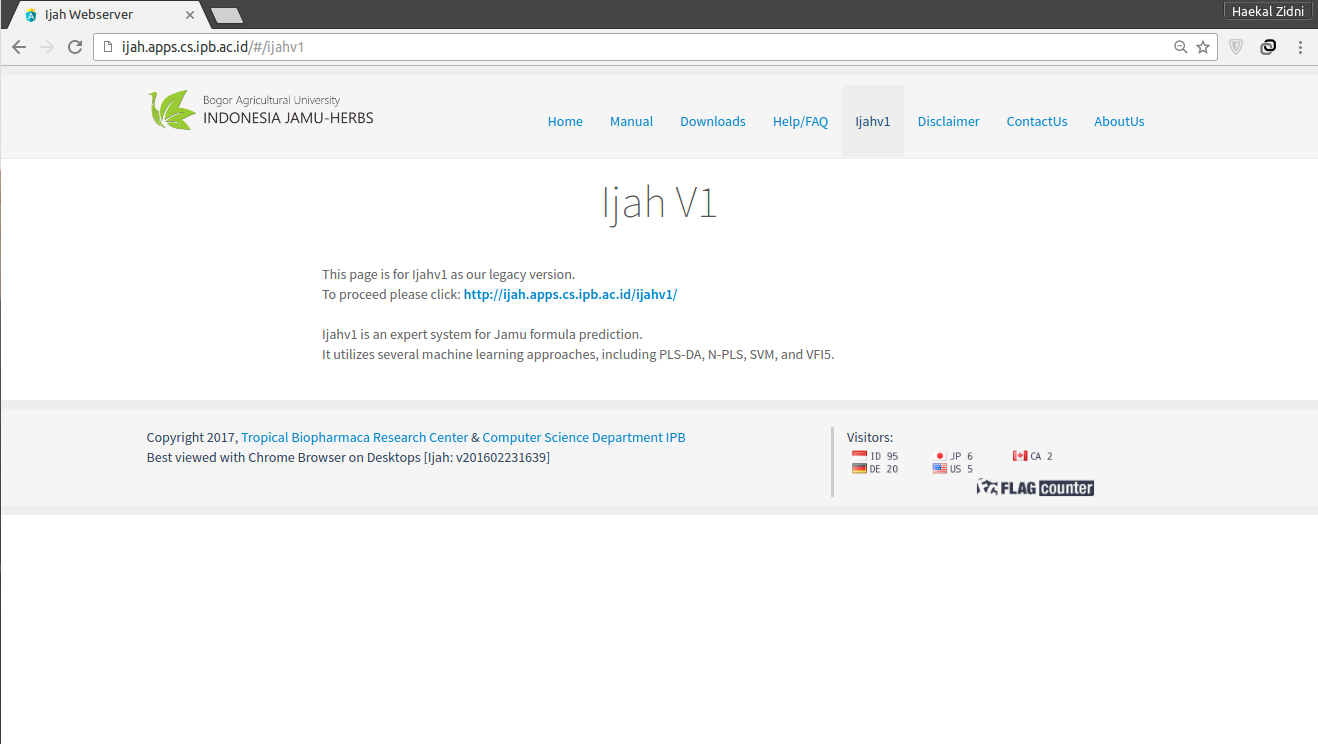
\includegraphics[scale=0.3]{ijah_v1.png}
% 	\caption{Isi halaman menu Ijah v1}
% 	\label{fig:ijah_v1}
% \end{figure}

% Jika anda ingin mengakses Ijah v1 silakan mengunjungi \url{http://ijah.apps.cs.ipb.ac.id/ijahv1/}

% \section{Disclaimer}

% Menu \emph{Disclaimer} berisikan pernyataan batasan responsibility pihak Ijah Webserver atas penggunaan hasil \emph{output} dari Ijah Webserver.

% \begin{figure}[H]
% 	\centering
% 	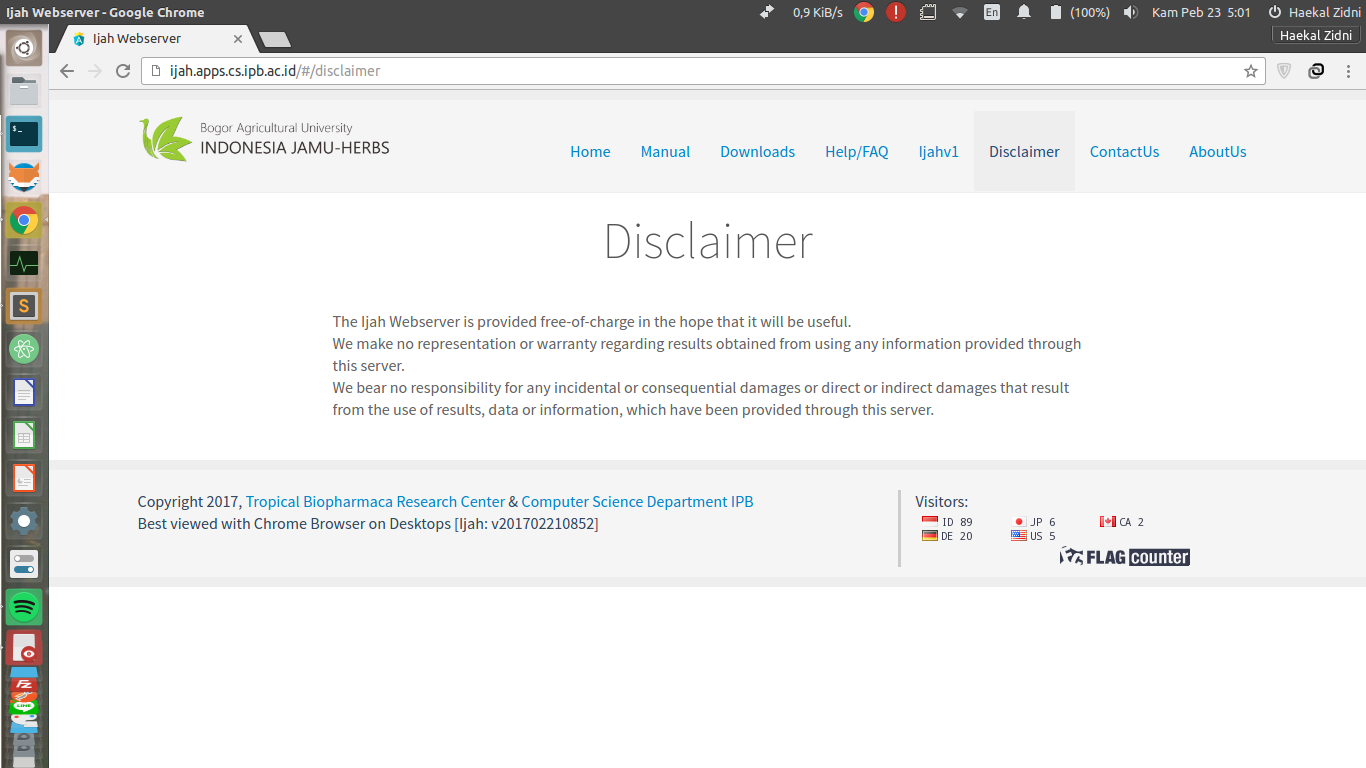
\includegraphics[scale=0.3]{ijah_disclaimer.png}
% 	\caption{Isi halaman Disclaimer}
% 	\label{fig:ijah_disclaimer}
% \end{figure}

% Di halaman ini kami menyatakan bahwa penggunaan Ijah Webserver ini gratis, dengan harapan dapat membantu banyak pihak. Namun kami tidak menjamin akibat dari penggunaan informasi dari Webserver ini. Dan kami tidak bertanggungjawab atas insiden atau kerusakan baik langsung maupun tidak langsung yang diakibatkan oleh penggunaan data atau informasi yang kami sediakan di Webserver ini.

% \section{Contact Us} \label{Contact Us}

% Menu \emph{Contact Us} merupakan sarana komunikasi antara pengguna dengan tim pengembang Ijah Webserver. Dengan mengisikan tanggapan/keluhan/saran pada form Contact Us, tanggapan anda akan terkirim ke E-mail kami.

% \begin{figure}[H]
% 	\centering
% 	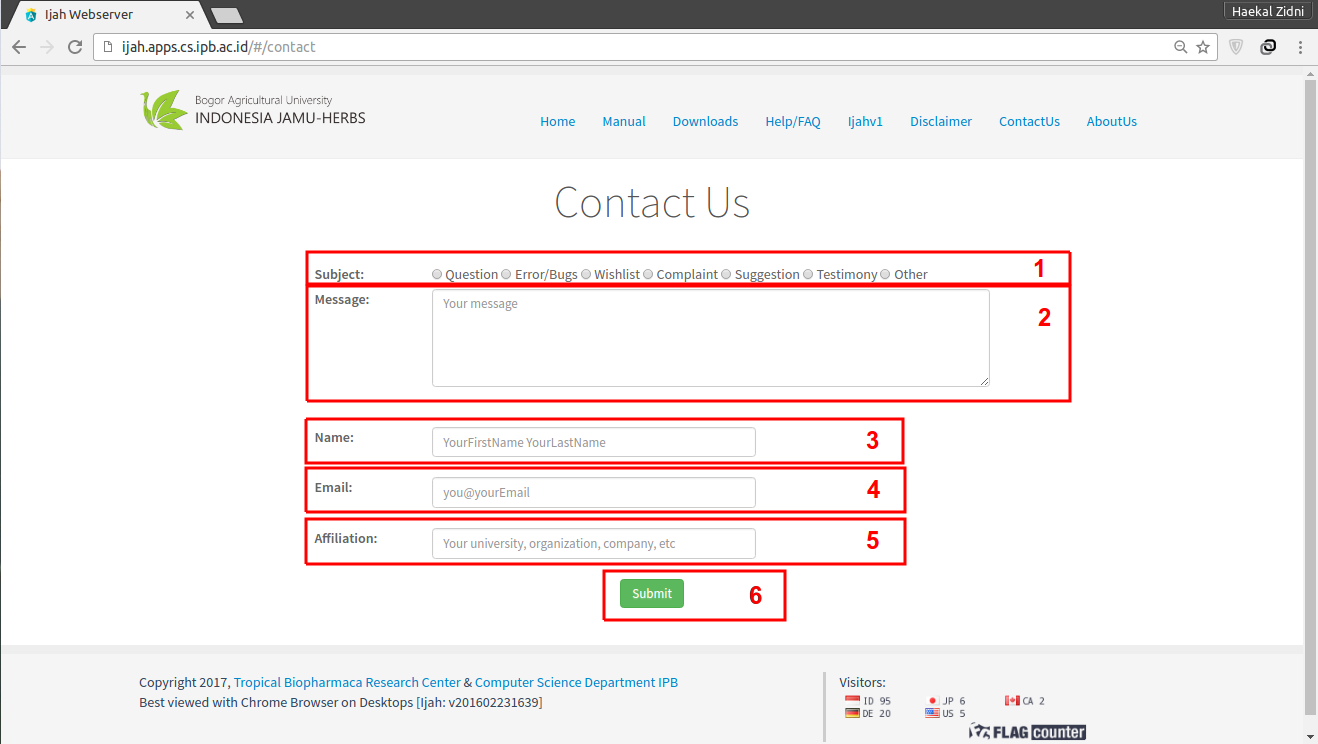
\includegraphics[scale=0.3]{ijah_contact_page.png}
% 	\caption{Halaman Contact Us pada Ijah Webserver}
% 	\label{fig:ijah_contact_page}
% \end{figure}

% \subsection{Subject}
% Pada bagian \emph{Subject} anda akan memilih jenis tanggapan anda, yaitu pertanyaan (Question), memberitahukan adanya kesalahan (Error/Bugs), menyampaikan saran fitur apa yang diinginkan pada versi selanjutnya (Wishlist), menyampaikan keluhan (Complaint), saran (Suggestion), memberikan testimoni tentang Ijah Webserver (Testimony), atau menyampaikan hal lain yang tidak termasuk dalam kategori diatas, dapat dikategorikan pada Other.

% \begin{figure}[H]
% 	\centering
% 	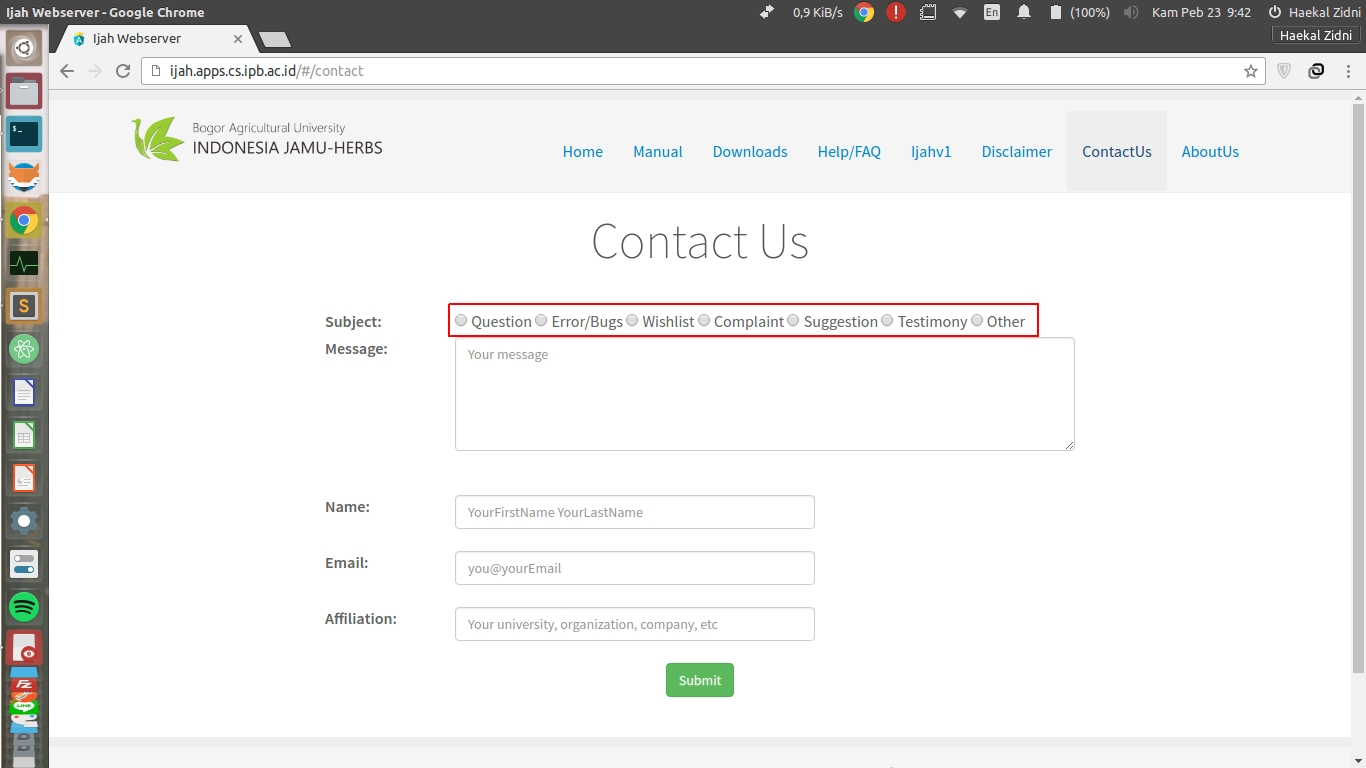
\includegraphics[scale=0.3]{ijah_contact_subject.png}
% 	\caption{Bagian \emph{Subject} pada menu Contact Us}
% 	\label{fig:ijah_contact_subject}
% \end{figure}

% \subsection{Message}
% Isikan pesan anda pada bagian \emph{Message}. Jumlah karakter tidak dibatasi, jadi mohon untuk tidak menggunakan singkatan jika tidak diperlukan demi memudahkan tim kami dalam membaca tanggapan anda. 

% \begin{figure}[H]
% 	\centering
% 	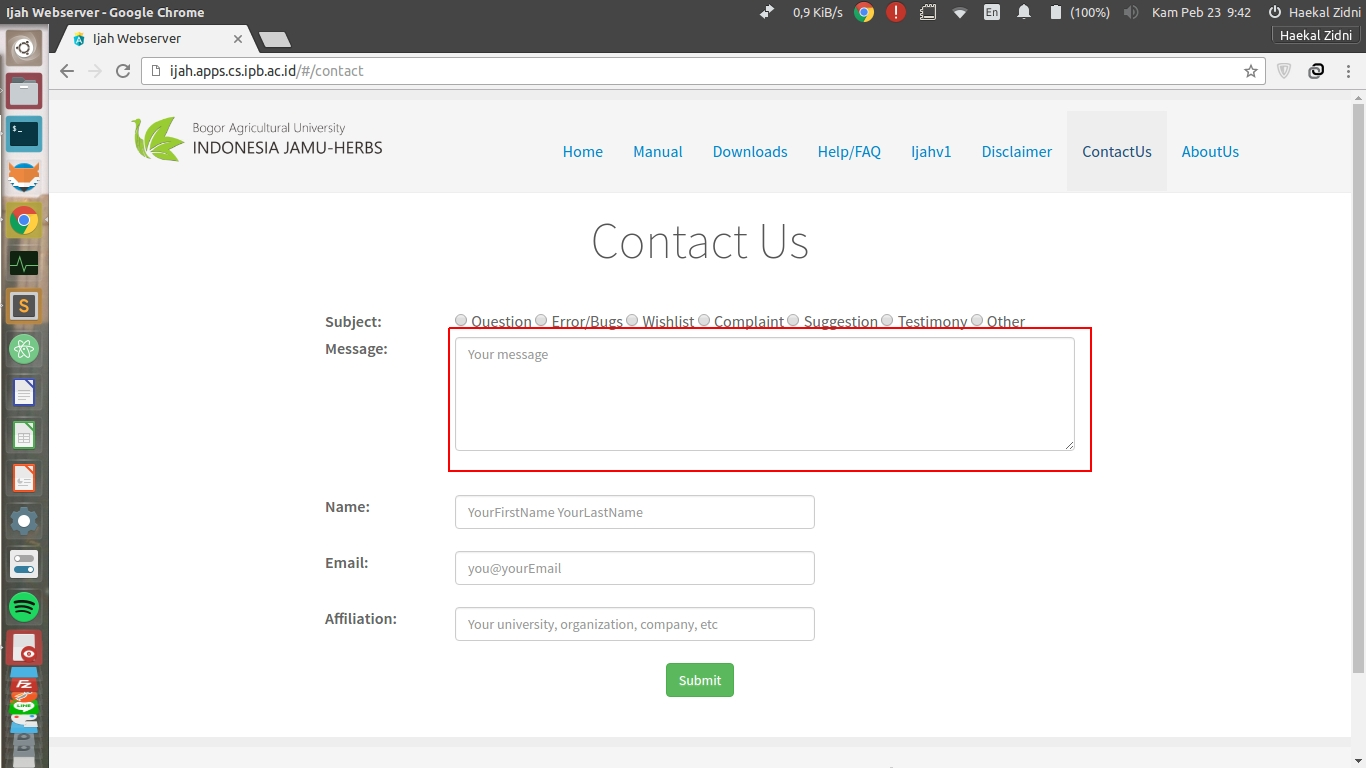
\includegraphics[scale=0.3]{ijah_contact_message.png}
% 	\caption{Bagian \emph{Message} pada menu Contact Us}
% 	\label{fig:ijah_contact_message}
% \end{figure}

% \subsection{Memasukkan Data Diri Anda}
% Setelah menuliskan tanggapan, silakan isi data diri anda, nama pada bagian \emph{Name}, alamat E\-mail anda pada bagian \emph{E\-mail}, dan afiliasi anda (organisasi, universitas, atau perusahaan) pada bagian \emph{Affiliation}.

% \textbf{Penting:} Nama dan alamat E-mail \emph{wajib} diisi. 

% \begin{figure}[H]
% 	\centering
% 	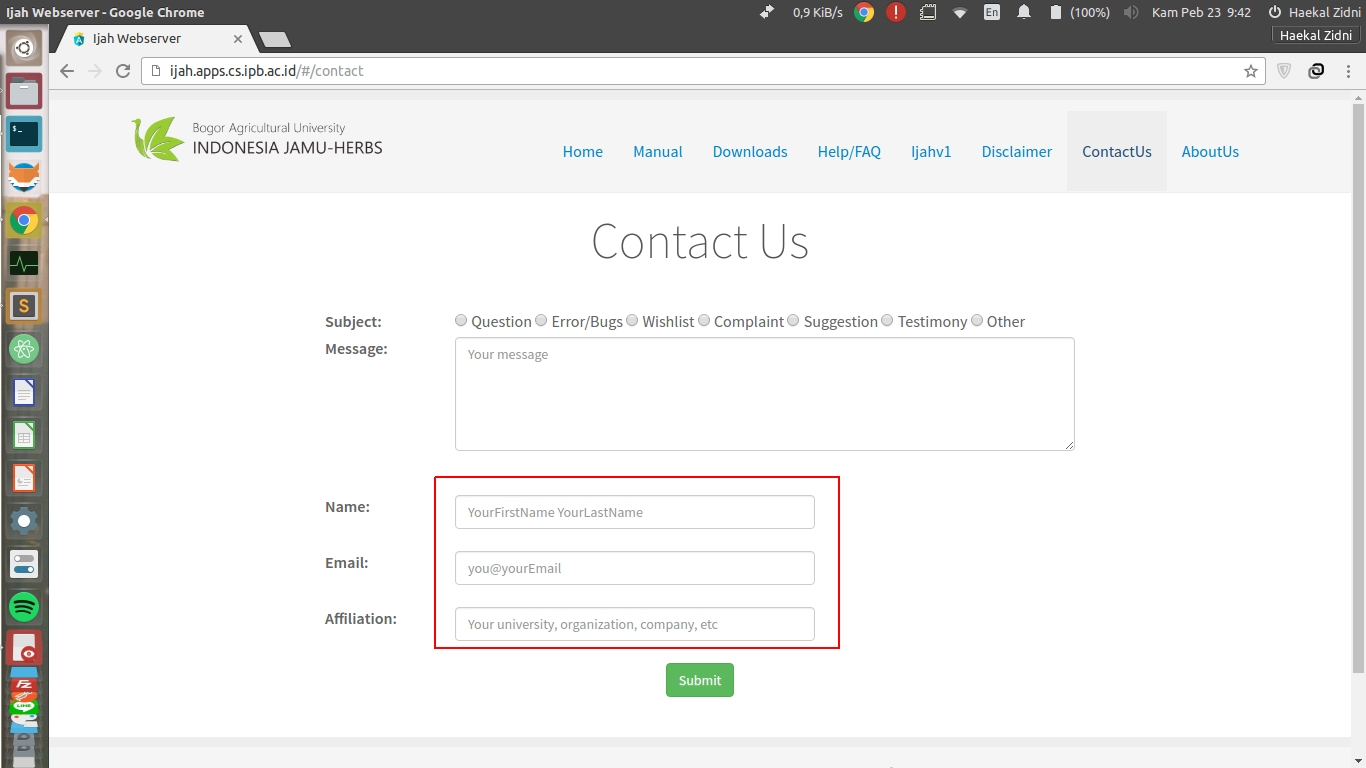
\includegraphics[scale=0.3]{ijah_contact_nameinput.png}
% 	\caption{Form pengisian nama, E-mail, dan afiliasi}
% 	\label{fig:ijah_contact_nameinput}
% \end{figure}

% Setelah terisi, tekan \textbf{Submit} dan tanggapan anda akan terkirim.

% \subsection{About Us}

% Menu \emph{About Us} berisi info tentang tim pengembang Ijah Webserver

% \begin{figure}[H]
% 	\centering
% 	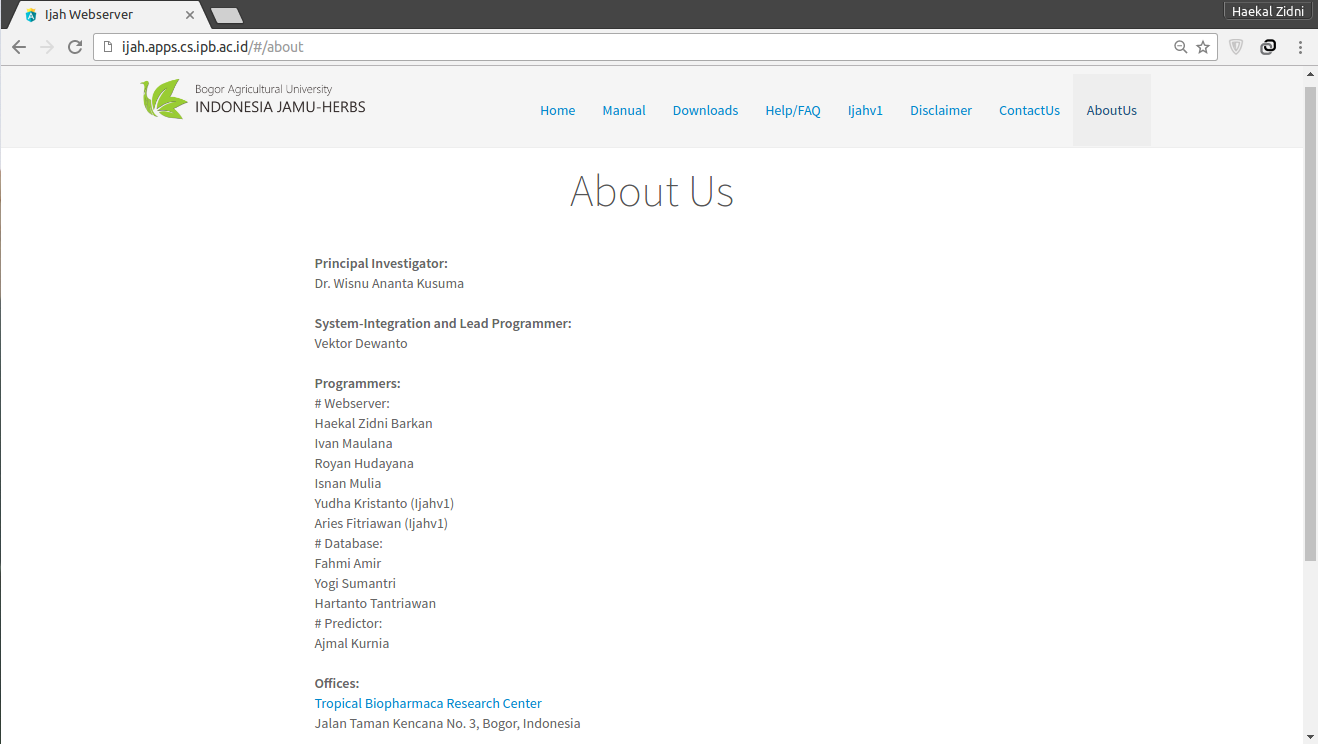
\includegraphics[scale=0.3]{ijah_about.png}
% 	\caption{Isi halaman About Us}
% 	\label{fig:ijah_about}
% \end{figure}